
\chapter{基于主导卷积核分解和知识预回归的模型加速}
\label{cha:acc}

\section{引言}
\label{sec:acc:introduction}

近年来,卷积神经网络在计算机视觉领域取得了重大研究突破,特别是在视觉物体识别~\cite{krizhevsky2012imagenet}、物体检测~\cite{girshick2014rich}和语义分割~\cite{sermanet2013overfeat}等视觉任务中。2012年,Krizhevsky~\cite{krizhevsky2012imagenet}凭借GPU强大的并行计算能力,在ImageNet大规模视觉物体识别挑战赛中一举夺冠。自此之后,卷积神经网络迎来了飞速发展的时期。然而,优越性能往往来自更深或更宽的网络结构和超大规模的计算。但是具有大规模参数的深度卷积网络模型,在测试阶段需要消耗大量的计算资源与时间,很难在实际生活中得到应用与推广。因为需要消耗大量的计算资源,应用无法部署在用户端;部署在服务器也很难应对大量并发的请求;此外用户也无法接受长时间的请求等待。为了解决这样的问题,早期工作主要集中在硬件相关的优化~\cite{vanhoucke2011improving,farabet2011large,krizhevsky2014one,krizhevsky2012imagenet,jia2014caffe},但是硬件的研究进展已经无法满足人们对计算资源的需求。尤其是在如今这样一个移动互联网时代,智能手机和平板电脑成为人们工作生活的主流产品,如何在一个低端CPU和少量内存的GPU上运行深度卷积网络模型,逐渐引起学术界的关注。

对一个计算繁重的深度卷积网络模型进行加速,一个直接有效的方法是模型压缩\cite{denil2013predicting,jaderberg2014speeding,denton2014exploiting,lebedev2014speeding,zhang2015efficient}, \cite{jaderberg2014speeding},基于矩阵的低秩分解,将一个大模型或一组模型压缩成为一个计算量小、推理速度快的模型 。另一个研究方向是Hinton等人~\cite{hinton2015distilling}提出了知识蒸馏,即用一个很深(宽)的教师网络去“教”(训练)一个相对较浅(窄)的学生网络\cite{hinton2015distilling,bucilu2006model,ba2014deep,romero2014fitnets}。

\begin{figure}[t]
\centering
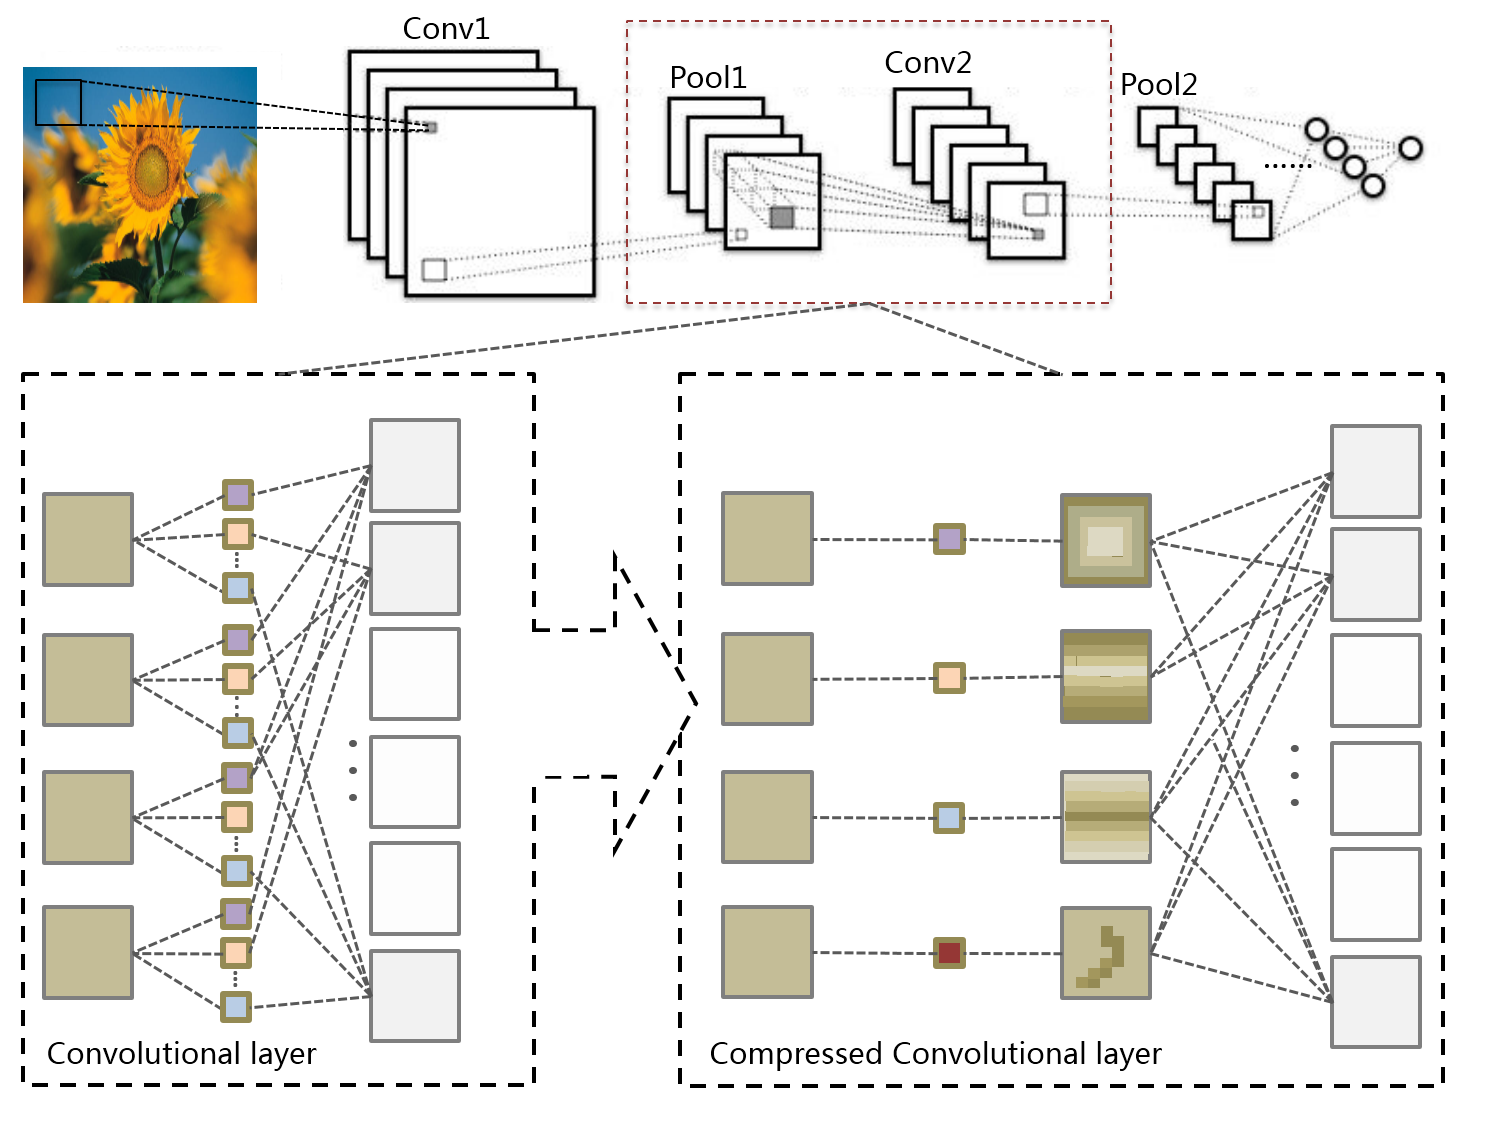
\includegraphics[width=1\columnwidth]{acc_old_intro.png}
\caption{主导卷积核参数压缩示意图。}
\label{fig:acc_old_intro}
\end{figure} 

受矩阵低秩分解~\cite{zhang2015efficient}启发,本章提出了一种新的基于主导卷积核(Dominant Convolutional Kernel,DK)分解的模型压缩方法,我们称之为DK分解。传统的卷积操作可以分解为两个步骤:特征提取和特征组合,在特征提取的过程中,通过挑选主导卷积核来缩减卷积参数,如图~\ref{fig:acc_old_intro}所示。模型压缩过程中,参数会大幅缩减,必然会引起网络性能的下降。受知识蒸馏~\cite{hinton2015distilling}思想启发,我们提出了知识预回归(Knowledge Pre-Regression,KP)的方法对压缩后的网络进行训练,尽量弥补网络因压缩所引起的精度损失。知识预回归是对FitNet~\cite{romero2014fitnets}训练方法的一种改进,采用全连接和交叉熵(Cross Entropy)损失函数来加速网络的收敛。知识预回归的训练方法有效地填补了教师网络与学生网络隐层特征之间的语义鸿沟。

本章采用主导卷积核(DK)分解的方法对大规模的教师网络进行压缩,采用知识预回归(KP)方法来训练压缩后的学生网络。我们将DK分解,KP训练的网络记为DK$^2$PNet,此网络有效地结合了目前主流的两种网络压缩方法。我们在四个数据集CIFAR-10~\cite{krizhevsky2009learning}、CIFAR-100~\cite{krizhevsky2009learning}、MNIST~\cite{lecun1998gradient}和SVHN~\cite{netzer2011reading}上对DK$^2$PNet进行了测试,与最近发表的很多CNN模型相比,DK$^2$PNet采用少量的参数,既可达到与其他模型接近的物体识别能力。

\section{相关工作}
\label{sec:acc:relate}

据我们了解,卷积模型加速的方法主要分为三个流派,分别是:模型压缩、知识蒸馏和硬件相关的加速方法。

模型压缩通过逐层地压缩卷积神经网络的参数,来实现模型的压缩与网络的加速。这种类型的方法通常由两部分组成,首先提出一种可以减少网络计算量的压缩方法,之后针对提出的压缩方法设计一种优化求解过程。对于优化求解,最常用的是卷积参数回归和数据回归两种方法。卷积参数回归,通过回归的方法直接重构卷积核参数。数据回归,通过回归的方式重构网络隐层的输出响应\cite{zhang2015efficient}。事实上,在模型压缩这个流派,压缩的方法往往受到更多的关注,其中基于矩阵低秩分解的方法是研究的热点之一。1989年,LeCun等人~\cite{lecun1989optimal}最早通过移除网络中不重要的权值参数,来实现网络加速的目的。Denil等人~\cite{denil2013predicting}证明了深度网络模型通常存在严重的过参数化(Over-Parameterization)现象,因此可以采用网络中一小部分参数子集去预测其他的参数。Jaderberg~\cite{jaderberg2014speeding} 进一步采用矩阵的低秩分解方法对网络的卷积层进行加速。他们采用两个秩为1的列向量对卷积核进行分解,逼近原有的卷积核。与此同时,Denton等人~\cite{denton2014exploiting}做了类似的工作,但是他们仅仅验证了这种分解方法在卷积网络的前两层的有效性。Lebedev等人~\cite{lebedev2014speeding}对四维卷积核在四个维度上进行了低秩分解,进一步压缩了网络的参数。Zhang等人~\cite{zhang2015efficient}在特征通道维度对卷积进行了分解,不同于以往的回归方法,对线性卷积核或线性输出特征进行回归,Zhang等人对网络的非线性激活响应进行回归。Chen等人~\cite{chen2015compressing} 提出了HashedNets,用散列去掉网络中固有的冗余信息。2016年,Iandola等人~\cite{iandola2016squeezenet}将卷积层替换为squeeze层和expand层,替换 $3\time3$ 的卷积核为 $1\time1$ 的卷积核并减少通道数,从而提出了SqueezeNet。Xception~\cite{chollet2016xception}是谷歌继Inception v3提出的一种改进,采用深层的分组卷积来替换Inception卷积。2017年,Howard等人\cite{howard2017mobilenets}提出Mobilenets,使用深层可分离的卷积来构建轻量级的深层神经网络,应用于移动和嵌入式设备。

另一种加速网络测试与预测时间的方法是基于知识蒸馏~\cite{hinton2015distilling}的训练方法,这种方法旨在通过用一个具有高识别率的教师网络去训练一个轻量的学生网络。知识蒸馏的概念是Hinton等人~\cite{hinton2015distilling}首次提出的,用于加快网络的预测时间。知识蒸馏是一种新颖的训练方法,将一个具有较高识别率的卷积网络网络中的“知识”进行压缩,迁移到被训练的目标网络。实际上,相似的想法早在2006年即被Bucilu$\check{a}$等人提及过,在他们的重要论文~\cite{bucilu2006model}中,成功地将多个复杂模型压缩成一个小的快速模型,并且没有引起明显的精度损失。与知识蒸馏类似,Ba和Caruana~\cite{ba2014deep}提出一个基于教师与学生网络体系结构的训练模型,他们证明了一个浅层网络也可以从深层网络模型中,学习到复杂的非线性映射关系,取得与深度网络近似的识别精度。Romero~\cite{romero2014fitnets}等人在这项工作的基础上,设计并成功训练出一个很深很瘦的网络FitNet,他们将知识蒸馏的理论从Softmax层推广到隐层,采用卷积回归的方式,将知识从教室网络的hint层,迁移到学生网络的guided层,提出了基于hint/guided结构的训练方法。

除此之外,与硬件相关的优化方法也可以加速网络,减少网络的预测时间。Vanhoucke等人~\cite{vanhoucke2011improving} 在低成本的x86 CPU上做了很多的优化工作,用于加速大规模矩阵运算。Farabet等人~\cite{farabet2011large}设计了适用于卷积运算的大规模FPGA集群。Krizhevsky~\cite{krizhevsky2014one}提出了一种新的适用于多GPU并行训练的并行化方法。cuda-convnet~\cite{krizhevsky2012imagenet}和caffe~\cite{jia2014caffe},两个开源的卷积神经网络计算框架,都提供了有效的GPU加速实现。此外,基于傅里叶变换,Mathieu等人~\cite{mathieu2013fast}将卷积操作从时域转换到频域,使得卷积操作加快了接近两倍。

\section{模型}
\label{sec:acc:model}

本节我们提出了基于主导卷积核(Dominant Convolutional Kernel,DK)分解的卷积压缩方法,和基于知识预回归(Knowledge Pre-Regression,KP)的网络训练方法,最后对两种方法与其他类似网络加速方法进行了分析与对比。

\subsection{主导卷积核}
\label{sec:acc:model:dk}

\begin{figure}
\centering
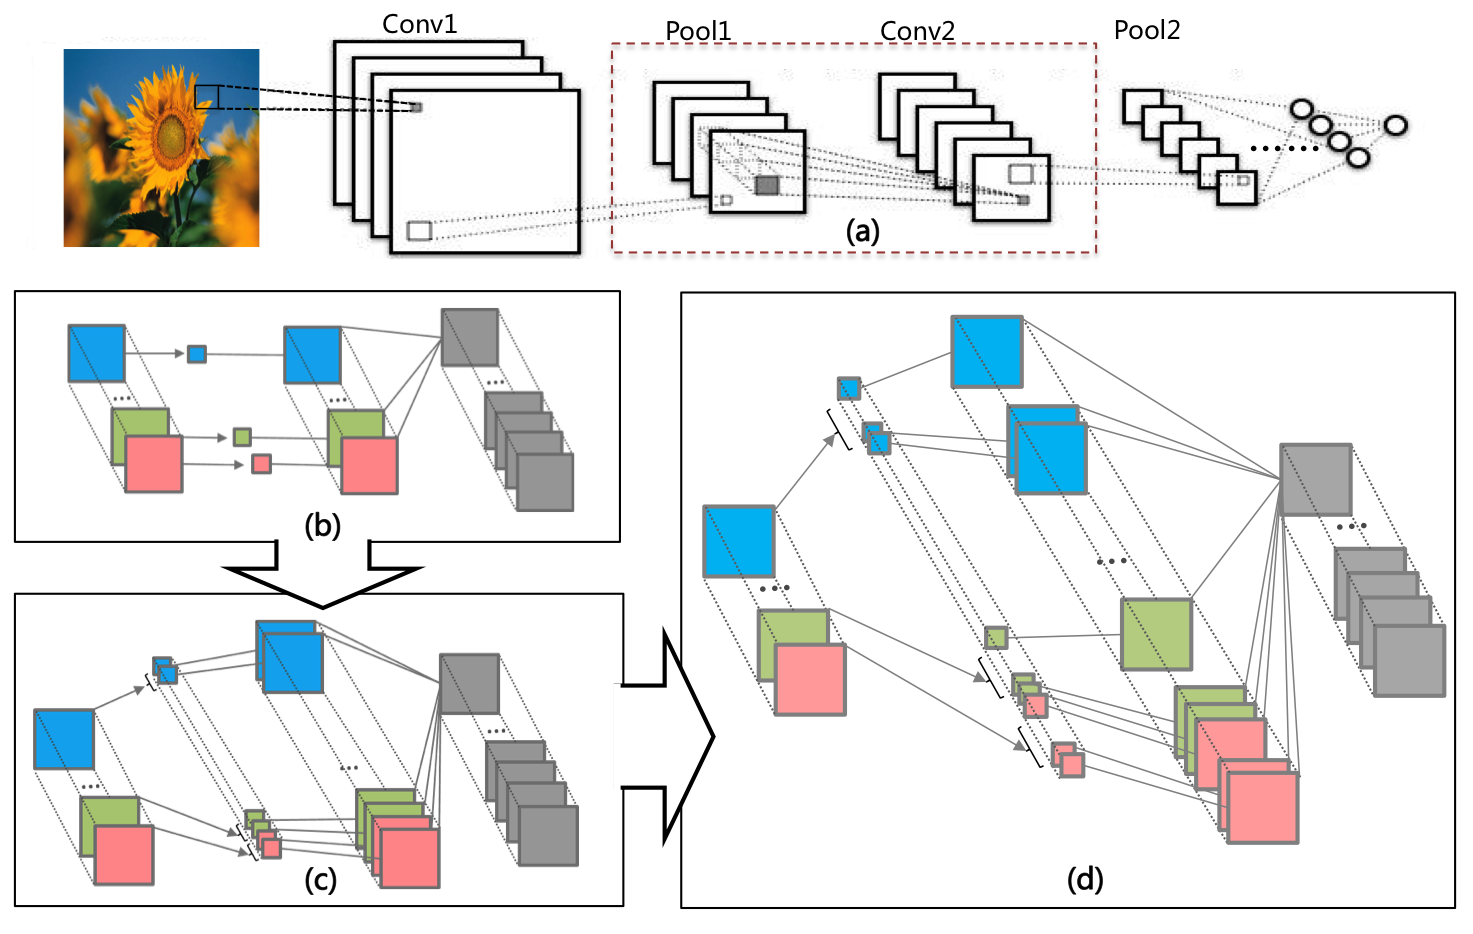
\includegraphics[width=1\columnwidth]{acc_dk.png}
\caption{主导卷积核。 (a) 传统卷积核;(b) 1比1情况下的主导卷积核;(c) 1比2情况下的主导卷积核;(d) 1比n情况下的主导卷积核。}
\label{fig:acc_dk}
\end{figure} 

在卷积神经网络中,具有大量参数的卷积操作对特征提取起到了至关重要的作用。实际上,大量的参数与计算量都集中在卷积层。因此对于卷积神经网络的压缩,最适合从卷积层参数压缩入手。因此,本节我们提出了基于主导卷积核分解的卷积参数压缩方法。

假设 $c_i$ 和 $c_o$ 分别代表卷积层输入和输出的通道数,$k_h$ 和 $k_w$ 分别代表卷积核的高度和宽度,对于传统的卷积方式,如图~\ref{fig:acc_dk} (a)所示,卷积核的大小为 $c_i{\times}c_o{\times}k_h{\times}k_w$。

卷积操作由乘法和加法运算组成,不同的卷积核与输入特征图的乘法操作可以理解为特征提取的过程,加法操作可以理解为特征组合的过程。将卷积操作理解为特征提取与特征组合,基于这样的观点,我们提出了主导卷积核分解,如图~\ref{fig:acc_dk} (b)(c)(d) 所示。以图~\ref{fig:acc_dk} (b)中1比1情况下的主导卷积核分解为例,对于每张输入特征图,我们只选择一个卷积核对其进行特征提取,再通过对所有特征进行线性加权的方式进行特征组合。特征提取可以通过分组卷积的方式实现,而特征选择可以通过使用具有 $1\times1$ 感受野大小的卷积操作实现。

对于传统的卷积方法如图~\ref{fig:acc_dk} (a)所示,每张输入特征图都和 $c_o$ 个卷积核进行卷积,对于图~\ref{fig:acc_dk} (b)中 1比1 情况下的主导卷积核,每个特征图只需要和一个卷积核进行卷积。上述过程可以推广到 1比2(如图~\ref{fig:acc_dk} (c)),1比$n$(如图~\ref{fig:acc_dk} (d))的情况,其中的 $n: 1{\le}n{\le}k_h{\times}k_w$ 称为主导卷积核的个数。在主导卷积核方法中,特征提取阶段的参数个数为 $n{\times}c_i{\times}k_h{\times}k_w$。在特征组合阶段,需要对所有特征提取阶段得到的中间结果进行线性加权,在特征选择阶段一共产生了$n{\times}c_i$ 组各不相同的特征,因此特征组合阶段需要的参数个数为 $n{\times}c_i{\times}c_o$。理论上说,当 $n$ 达到最大值 $k_h{\times}k_w$ 的时候,主导卷积核与传统的卷积等价。这是因为在线性代数理论中, $k_h{\times}k_w$ 个线性独立的特征向量构成了 $k_h{\times}k_w$ 维线性空间的一组基。

根据上述分析,主导卷积核分解的参数个数为  $n{\times}c_i{\times}k_h{\times}k_w+n{\times}c_i{\times}c_o$,是传统卷积参数个数的 $n/c_o+n/(k_h{\times}k_w)$ 倍。以一个常见的卷积层配置为例,对于一个具有 $3{\times}3$ 感受野大小,输入通道数为 96,输出通道数也为 96 的卷积层,主导卷积核仅需要 12\%(1比1情况)或 24\%(1比2情况)的参数规模。而卷积层的计算量与卷积层的参数个数是成正比的,因此采用主导卷积核对卷积层进行压缩,可以极大地提高网络的计算速度,减少运行时间。主导卷积核的个数 $n$ 可以用于平衡卷积层的特征提取能力和计算复杂度。

\subsection{知识预回归}
\label{sec:acc:model:kp}

\begin{figure}[t]
\centering
\centerline{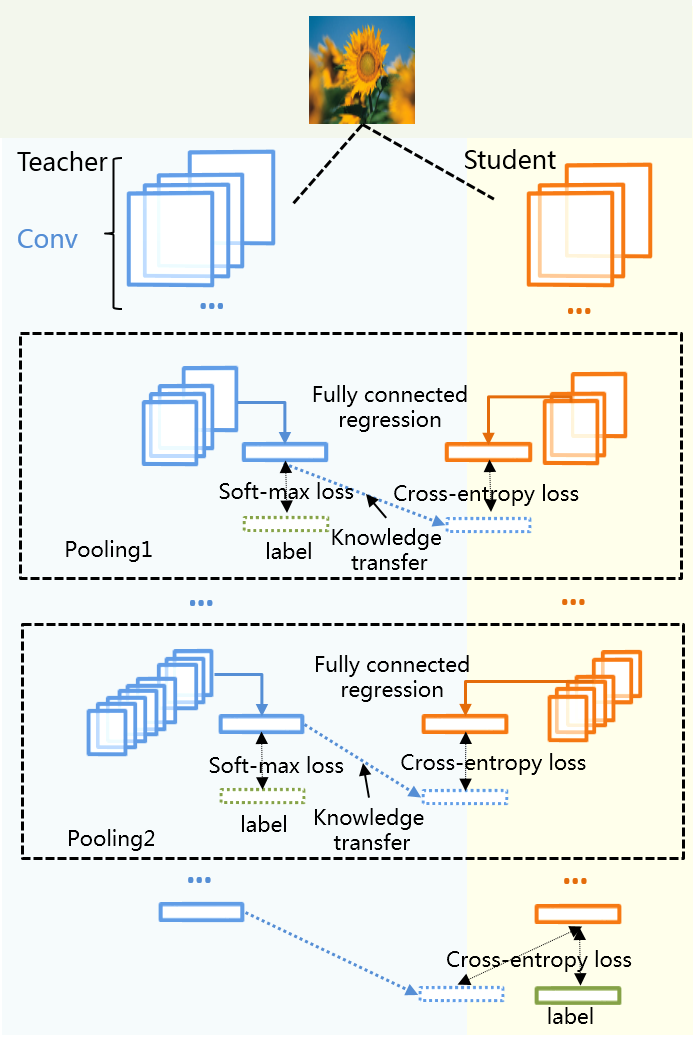
\includegraphics[height=1\columnwidth]{acc_old_kp.png}}
\caption{知识预回归。}
\label{fig:acc_kp}
\end{figure} 

知识蒸馏是2012年Hinton等人~\cite{hinton2015distilling}提出,用于将教师网络中的知识进行压缩,并迁移到学生网络的新型网络训练方法。网络的知识通常以网络参数的形式存储于卷积神经网络中,参数形式的知识太过于抽象以至于很难进行知识的迁移。Hinton等人将知识定义为一种从输入图像到目标类别概率(即Softmax层的输出)的非线性映射,知识迁移的最初的方式就是,将教师网络得到的概率分布迁移到学生网络。在第~\ref{sec:sam:vis}中可视化操作中,我们同样发现,哪怕对于错误的分类结果,卷积网络输出的概率分布仍然具有很大的参考价值。Romero等人~\cite{romero2014fitnets}将知识蒸馏的思想扩展到教师网络与学生网络的隐层,采用卷积回归的方式匹配隐层特征维度,再通过L2损失函数来回归对应隐层的激活响应。在此工作的基础上,本节提出了知识预回归方法对训练教师网络和学生网络进行知识回归。与Romero不同的是,我们在教师网络的隐层增加了一个额外的分类器,用于生成目标类别的概率分布,进一步采用交叉熵损失函数为优化目标,对学生网络的隐层特征进行回归,如图~\ref{fig:acc_kp}所示。实验结果表明,知识预回归相对于FitNet方法,更加稳定鲁棒,具有更快的收敛速度。

我们采用与~\cite{romero2014fitnets}相同的表述方式,即采用hint/guided对分别表示教师网络和学生网络对应的隐层对。通过DK分解对教师网络进行压缩,得到学生网路。因此,教师网络和学生网络具有相似的结构,但学生网络卷积层的特征拟合能力相对要若很多。采用逐层回归的方式对两个网络进行知识预回归往往难以起到较好的训练效果,根据我们的经验,选择对应的池化层作为hint/guided对进行知识预回归,可以有效地加快网络的收敛速度,提高学生网络的泛化能力。

选定的hint/guided对通常具有不同的特征维度,Romero等人~\cite{romero2014fitnets} 采用卷积回归来匹配特征维度,采用L2损失函数进行特征回归,这种方式虽然很简单,但是却很难收敛。我们采用知识预回归的方式来解决FitNet存在的不稳定和收敛慢等问题,如图~\ref{fig:acc_kp}所示。我们在 hint 层引入一个辅助分类器,该分类器由一个具有参数 $R_t$ 的全连接层,和一个 Softmax 层组成,采用图像真实的类别标签 $l$ 监督优化 $R_t$。该分类器的中间结果,会产生目标类别的概率分布 $b_t$,将此概率分布迁移到对应的guided层,来实现隐层知识的回归。类似地,对于学生网络,我们引入了另外一个辅助分类器,该分类器由一个以 $R_s$ 为参数的全连接层,和交叉熵函数组成。通过两个辅助分类器来建立hint层与guided层之间的联系,知识预回归的损失函数可以公式化表示为:
\begin{align} \label{equ:bridge}
\mathcal{L}_{KB}(W_s, R_t, R_s)={\lambda}\mathcal{H}(b_t^{\tau}, b_s^{\tau})+\mathcal{S}(l, b_t)
\end{align}
\begin{align} \label{equ:bt}
%b_t^{\tau}=\mathit{softmax}(\frac{{R_t}H_t}{\tau})
b_t^{\tau}=\mathit{softmax}(\frac{h(x; W_t, R_t)}{\tau})
\end{align}
\begin{align} \label{equ:bs}
%b_s^{\tau}=\mathit{softmax}(\frac{{R_s}G_s}{\tau})
b_s^{\tau}=\mathit{softmax}(\frac{g(x; W_s, R_s)}{\tau})
\end{align}
其中 $\mathcal{S}$ 和 $\mathcal{H}$ 分别代表 Softmax 和交叉熵损失函数;$h$ 和 $g$ 分别代表从输入图像 $x$ 到 hint 和 guided 层输出特征的非线性映射;$W_t$ 和 $W_s$ 分别指代教师网络和学生网络的参数;温度参数(Temperature Parameter)$\tau$~\cite{hinton2015distilling}用来弱化特征类别的概率分布;${\lambda}$ 用于调节两个损失函数的权重。

我们通过最小化下面这个公式来训练整个网络:
\begin{align} \label{equ:all}
%\mathcal{L}(W_s, R_t^{(1{\cdots}n)}, R_s^{(1{\cdots}n)})={\lambda}\mathcal{H}(p_t^{\tau}, p_s^{\tau}) + \mathcal{H}(l, p_s) + \sum_{i=1{\cdots}l}{\lambda}_i\mathcal{H}(b_t^{\tau^{(i)}}, b_s^{\tau^{(i)}})+\mathcal{S}(l, b_t^{(i)})
\mathcal{L}(W_s)={\lambda}\mathcal{H}(p_t^{\tau}, p_s^{\tau}) + \mathcal{S}(l, p_s) + \sum_{i=1{\cdots}P}{\lambda}_i\mathcal{H}(b_t^{\tau^{(i)}}, b_s^{\tau^{(i)}})+\mathcal{S}(l, b_t^{(i)})
\end{align}
其中 $p_t$ 和 $p_s$ 分别是教师网络和学生网络的目标类别概率分布;$P$ 代表我们选择的对应 hint/guided 层。在我们的实验中,我们选择了前两个池化层作为 hint/guided 层,用于知识预回归。

\subsection{分析与讨论}
\label{sec:acc:model:discuss}

\begin{figure}
\begin{center}
\centerline{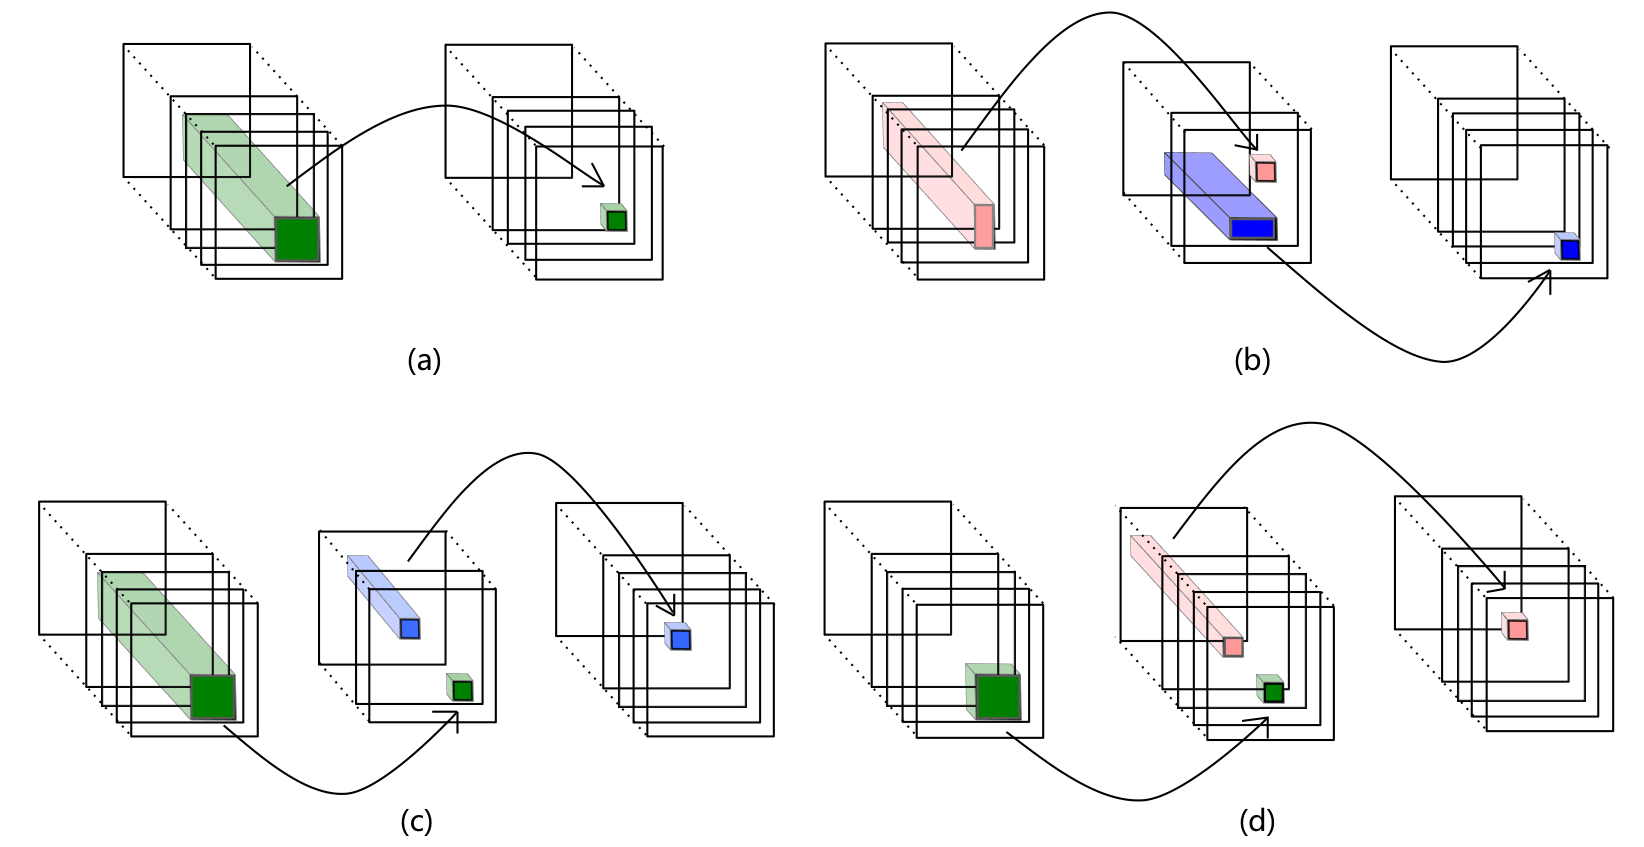
\includegraphics[width=1\linewidth]{acc_cmp.png}}
\caption{主导卷积核与其他压缩方法的对比。(a) 传统卷积操作;(b) Jaderberg~\cite{jaderberg2014speeding}的压缩方法;(c) Zhang~\cite{zhang2015efficient}的压缩方法;(d) 主导卷积核分解。}
\label{fig:acc_cmp}
\end{center}
\end{figure} 

第~\ref{sec:acc:model:dk}节中我们提出了基于主导卷积核分解的卷积分解方法,可以有效地压缩网络的参数,降低网络的计算量。尽管主导卷积核也是基于矩阵低秩分解的方法,但是与Jaderberg~\cite{jaderberg2014speeding}和Zhang~\cite{zhang2015efficient} 的方法不同,如图~\ref{fig:acc_cmp}所示。Jaderberg等人将传统的卷积操作分解为两次低秩线性映射,即对于原始的输入图像,分别采用具有 $1{\times}d$ 和 $d{\times}1$ 感受野大小的卷积核对其卷积参数进行分解。Zhang等人也采用两步分解,不同的是他们在通道上对卷积核进行了低秩分解。我们提出的主导卷积核如图~\ref{fig:acc_cmp}(d)所示,与Zhang等人的方法类似,也是在通道上对卷积核进行分解,与其不同的是,我们采用分组卷积的方式来降低特征维度,减少卷积参数与计算量。

为了加快被压缩网络的收敛速度,提高网络的泛化能力,我们提出了知识预回归的训练方法。在Hinton~\cite{hinton2015distilling}和Romero~\cite{romero2014fitnets}等人工作的基础上,我们对知识蒸馏和FitNet进行了拓展,如图\ref{fig:acc_kp}所示。知识预回归的训练结构看起来像两个并行的DSN~\cite{lee2015deeply}网络模型,但是他们具有不同的含义。DSN通过在隐层引入所谓的伴随优化目标来提高单个网络的特征表达能力,而知识预回归更多的关注于教师网络知识的压缩、提取与迁移。知识预回归方法使得学生网络可以学习到教师网络的特征表达能力与泛化能力。

\section{实验结果}
\label{sec:acc:experiment}

在开源项目caffe~\cite{jia2014caffe}基础上,我们对DK$^2$PNet网络进行了测试。所有的实验均运行于具有两颗GPU核心的单卡K80高性能服务器。在CIFAR-10~\cite{krizhevsky2009learning},CIFAR-100~\cite{krizhevsky2009learning},MNIST~\cite{lecun1998gradient}和 SVHN~\cite{netzer2011reading}四个数据集上,DK$^2$PNet均可以采用较少的模型参数与计算量达到一个较高的物体识别率。在CIFAR-10数据集上,我们进行了更多的实验来验证DK$^2$PNet方法的有效性。

在所有的实验中,我们均采用批大小(Batch Size)为96的批量随机梯度下降法来更新网络参数。网络的初始学习率设置为0.01,训练过程中当损失函数无法继续降低时对学习率进行调整,减小 10 倍,持续减小学习率三次,直到学习率减小到1e-5,所有卷积层偏执项的学习率均设为正常学习率的2倍。整个训练过程中,均采用 0.9 的动量因子(momentum)和 0.004 的权重衰减因子(weight decay)。在知识预回归的损失函数中(公式~\ref{equ:all}),参数$\lambda$,${\lambda}_1$ 和 ${\lambda}_2$的取值范围是[0.0001, 1],例如对于Softmax层 $\lambda=0.1$,第二个池化层 ${\lambda}_1=0.01$,第一个池化层 ${\lambda}_2=0.001$,即为一组有效的参数。对于每个数据集,我们均采用逐像素地减去训练样本像素均值的方式对图像进行预处理。

\subsection{网络结构}
\label{sec:acc:experiment:arc}

\begin{table}[t]
\begin{center}
\caption{基于主导卷积核分解的DK$^2$PNet-96网络识别性能对比。}
\label{tab:fit}
\begin{tabular}{L{5cm}C{2cm}C{3cm}}
 \toprule[1.5pt]
 {\heiti 模型} & {\heiti 参数个数} & {\heiti 测试错误率(\%)} \\
 \midrule[1pt]
 CNN-96 & 0.75 M & 7.82 \\
 \hline
 DK$^2$PNet-96(1比1,SGD)& 0.09 M & 9.59 \\
 DK$^2$PNet-96(1比2,SGD)& 0.18 M & 8.98 \\
 DK$^2$PNet-96(1比3,SGD)& 0.28 M & 8.55 \\
 DK$^2$PNet-96(1比4,SGD)& 0.37 M & 8.26 \\
 DK$^2$PNet-96(1比5,SGD)& 0.46 M & {\bf 7.98} \\
 DK$^2$PNet-96(1比6,SGD)& 0.55 M & 8.25 \\
 DK$^2$PNet-96(1比7,SGD)& 0.64 M & 8.56 \\
 DK$^2$PNet-96(1比8,SGD)& 0.73 M & 8.21 \\
 DK$^2$PNet-96(1比9,SGD)& 0.82 M & 8.03 \\
  \bottomrule[1.5pt]
\end{tabular}
\end{center}
\end{table}

本节中我们设计了一组结构相似但参数规模不同的网络。假设所有的卷积层,不论是传统卷积层还是主导卷积核卷积层,都具有相同的输入输出特征通道数 $K$,方便意见,采用与~\cite{liang2015recurrent}相同的符号表示,即CNN-$K$ 或者 DK$^2$PNet-$K$ 。其中CNN-$K$是教师网络,采用传统的卷积层,每个卷积层都具有 $K$ 个特征通道;DK$^2$PNet-$K$ 与 CNN-$K$ 结构类似,但是将其中的传统卷积层替换为主导卷积核卷积层,并采用知识预回归的方法进行网络训练。

教师网络CNN-$K$是一个具有 11 层结构的卷积网络模型,包括 10 个卷积层和 1 个全连接层。在网络的第 2 层、第 6 层和第 10 层之后,各接了一个池化层。最后采用Softmax层生成网络的目标概率。

学生网络DK$^2$PNet-$K$是对教师网络CNN-$K$进行主导卷积核分解得到的,具有与教师网络相类似的结构。对于第一个卷积层,输入图片最多具有3个通道,采用主导卷积核分解对该层压缩程度有限,因此对于第一个卷积层,并不对其进行压缩。对于CNN-$K$的第二到最有一个卷积层,采用主导卷积层替换传统卷积层,即得到DK$^2$PNet-$K$。

对于所有的卷积层,不论是传统卷积还是主导卷积,均采用 $3\times3$ 大小的感受野和 1 个像素的边界扩充和卷积滑动步长,这样可以保证输出和输入特征图具有相同的维度。对于前两个池化层,我们采用具有 $2\times2$ 感受野大小,步长为 2 的均值池化;最后一个池化层是全局均值池化。此外,所有的卷积层之后都采用BN层对卷积输出进行批正则化,采用ReLU作为非线性激活函数,采用Dropout来防止网络多拟合。对于DK2PNet-$K$(1比1)学生网络,一共具有 $(9K^2+108K)$ 个参数,而教师网络CNN-$K$的参数个数为$(81K^2+27K)$。


\subsection{CIFAR-10}
\label{sec:acc:experiment:cifar10}

CIFAR-10~\cite{krizhevsky2009learning}是Krizhevsky搜集并标注的一个图像识别数据集,具有 60,000 张 $32\times32$ 的彩色图片。

\begin{table} [t]
\begin{center}
\caption{知识预回归与梯度下降性能对比。}
\label{tab:kp}
\begin{tabular}{L{5cm}C{2cm}C{3cm}}
 \toprule[1.5pt]
 {\heiti 模型} & {\heiti 参数个数} & {\heiti 测试错误率(\%)} \\
 \midrule[1pt]
\multicolumn{3}{c}{\heiti 随机梯度下降} \\
\hline
DK$^2$PNet-96 (1比1, BN) & 0.09 M & {9.59} \\
DK$^2$PNet-96 (1比2, BN) & 0.18 M & {8.98} \\
DK$^2$PNet-128 (1比2, BN) & 0.32 M & {8.31} \\
DK$^2$PNet-160 (1比2, BN) & 0.49 M & {7.91} \\
 \midrule[1pt]
\multicolumn{3}{c}{\heiti 知识预回归} \\
\hline
高性能教师网络 & 0.75 M & 7.82 \\
DK$^2$PNet-96 (1比1, BN) & 0.09 M & {9.52} \\
DK$^2$PNet-96 (1比2, BN) & 0.18 M & {8.73} \\
DK$^2$PNet-128 (1比2, BN) & 0.32 M & {7.90} \\
DK$^2$PNet-160 (1比2, BN) & 0.49 M & {7.60} \\
\hline
低性能教师网络 & 0.75 M & 12.18 \\
DK$^2$PNet-96 (1比1, BN) & 0.09 M & {9.57} \\
DK$^2$PNet-96 (1比2, BN) & 0.18 M & {8.78} \\
DK$^2$PNet-128 (1比2, BN) & 0.32 M & {7.96} \\
DK$^2$PNet-160 (1比2, BN) & 0.49 M & {7.70} \\
  \bottomrule[1.5pt]
\end{tabular}
\end{center}
\end{table}

首先,我们通过一组对比实验来测试第~\ref{sec:acc:model:dk}节中主导卷积核分解对网络识别能力的影响,如表~\ref{tab:fit} 所示。其中网络CNN-96是本组对比实验的基准网络,该网络也是后文中将要用到的教师网络,具有不同压缩比的DK$^2$PNet-96作为对比研究对象。我们对九组DK$^2$PNet-96进行了测试,为了对比的公平,所有十个网络模型采用梯度下降算法进行训练,而没有引入知识预回归的训练策略,这里我们将采用梯度下降方法训练的DK$^2$PNet-96记为DK$^2$PNet-96(SGD)。实验结果如表~\ref{tab:fit} 所示,其中具有1比1压缩比的DK$^2$PNet-96仅仅采用 0.09M 参数,即达到了 9.59\% 的测试错误率,这有可能是CIFAR-10上测试误差低于 10\% 的最小模型。通过增大主导卷积核的个数降低压缩比,DK$^2$PNet-96 的识别率会逐渐提高,最好的压缩比率是1比5,此时 DK$^2$PNet-96 取得了 7.98\% 的测试错误率。意外的是,理论上与 CNN-96 等价,参数数量比 CNN-96 还要多的具有1比9压缩比的DK$^2$PNet-96,识别能力反而不如 CNN-96,我们猜测这可能是由网络参数冗余而产生的过拟合问题,影响了网络的泛化能力。


更进一步,我们设计了另外一组实验来验证第~\ref{sec:acc:model:kp}节中,知识预回归对网络性能的提升。我们将知识预回归方法与批量随机梯度下降方法进行了对比,实验结果如表~\ref{tab:kp} 所示。表~\ref{tab:kp} 中,四个具有不同压缩比和参数规模的DK$^2$PNet网络分别采用梯度下降法和知识预回归法进行训练。对于知识预回归训练方法,我们选取了测试误差率为 7.82\% 和 12.18\% 的两个教师网络分别训练学生网络。实验结果表明,在四组对比模型上,采用知识预回归的方法训练出的网络在最终的识别能力上都强于随机梯度下降的训练结果。对于具有1比1压缩比的DK$^2$PNet,知识预回归训练对其精度的提升非常有限,这是因为网络参数规模太小,网络的识别能力和泛化能力很难进一步提升。当测试网络的参数逐渐增加时,知识预回归对网络性能提升的幅度也会提高。此外我们还发现,相比于随机梯度下降法,即使我们用一个相对识别率较低的教师网络去训练学生网络,学生网络的识别率也是会受到影响的。当然,高性能的教师网络对学生网络的帮助更大。

\begin{table} [t]
\caption{正则化方法对DK$^2$PNet网络性能的影响。}
\label{tab:norm}
\begin{center}
\begin{tabular}{L{5cm}C{2cm}C{3cm}}
 \toprule[1.5pt]
 {\heiti 模型} & {\heiti 参数个数} & {\heiti 测试错误率(\%)} \\
 \midrule[1pt]
CNN-96 (LRN) & 0.75 M & 12.18 \\
DK$^2$PNet-96 (1比1, LRN) & 0.09 M & 26.88 \\
DK$^2$PNet-96 (1比2, LRN) & 0.18 M & 26.52 \\
DK$^2$PNet-128 (1比2, LRN) & 0.32 M & 25.01 \\
\hline
CNN-96 (BN) & 0.75 M & 7.82 \\
DK$^2$PNet-96 (1比1, BN) & 0.09 M & 9.59 \\
DK$^2$PNet-96 (1比2, BN) & 0.18 M & 8.98 \\
DK$^2$PNet-128 (1比2, BN) & 0.32 M & 8.31 \\
  \bottomrule[1.5pt]
\end{tabular}
\end{center}
\end{table}

正则化方法对网络的性能具有至关重要的影响,DK$^2$PNet可以在参数很少的情况下,取得如此卓越的识别能力,很大程度上要归功于批正则化(Batch Normalization,BN)~\cite{ioffe2015batch}方法。关于正则化对网络性能的影响,我们在CNN-96和DK$^2$PNet上进行了两组实验,一组采用批正则化方法,另一组采用局部响应正则化方法(Local Response Unit,LRN),对比结果如表~\ref{tab:norm} 所示。显然,批正则化方法的性能远远优于局部响应正则化方法,可见正则化方法对网络性能的提升起到了重要的作用。实际上,应用于池化层的知识预回归训练,在一定程度上也起到正则化的作用,通过回归的方式,强制学生网络的去学习教师网络的特征提取方式与泛化能力。

\begin{table} [!h]
\begin{center}
\caption{CIFAR-10数据集上与已知模型的对比试验。}
\label{tab:cifar10}
\begin{tabular}{L{5cm}C{2cm}C{3cm}}
 \toprule[1.5pt]
 {\heiti 模型} & {\heiti 参数个数} & {\heiti 测试错误率(\%)} \\
 \midrule[1pt]
\multicolumn{3}{c}{\heiti 没有数据增广} \\
\hline
\noalign{\smallskip}
Maxout~\cite{goodfellow2013maxout} & $>$5 M & 11.68 \\
Prob maxout~\cite{springenberg2013improving} & $>$5 M & 11.35 \\
NIN~\cite{lin2013network} & 0.97 M & 10.41 \\
DSN~\cite{lee2015deeply} & 0.97 M & 9.69 \\
RCNN~\cite{liang2015recurrent} & 1.86 M & 8.69 \\
ALL-CNN~\cite{springenberg2014striving} & 1.4 M & 9.08 \\
Tree+Max-Avg~\cite{lee2015generalizing} & 1.85M & \bf{7.62} \\
\hline
\noalign{\smallskip}
Teacher (CNN-96) & 0.75 M & 7.82 \\
DK$^2$PNet-96 (1比1) & 0.09 M & 9.52 \\
DK$^2$PNet-96 (1比2) & 0.18 M & 8.73 \\
DK$^2$PNet-128 (1比2) & 0.32 M & {7.90} \\
DK$^2$PNet-160 (1比2) & 0.49 M & \bf{7.60} \\
 \midrule[1pt]
\multicolumn{3}{c}{\heiti 具有数据增广} \\
\hline
Maxout~\cite{goodfellow2013maxout} & $>$5 M & 9.38 \\
dasNet~\cite{stollenga2014deep} &  $>$5 M & 9.22 \\
Prob maxout~\cite{springenberg2013improving} & $>$5 M & 9.39 \\
DropConnect~\cite{wan2013regularization} & - & 9.32 \\
NIN~\cite{lin2013network} & 0.97 M & 8.81 \\
DSN~\cite{lee2015deeply} & 0.97 M & 8.22 \\
RCNN~\cite{liang2015recurrent} & 1.86 M & 7.09 \\
Highway Network~\cite{srivastava2015training} & 2.3 M & 7.54 (7.72${\pm}$0.16) \\
ALL-CNN~\cite{springenberg2014striving} & 1.4 M & 7.25 \\
ResNet~\cite{he2015deep} & 1.7M & {6.43 (6.61${\pm}$0.16)} \\
Fitnet4-LSUV~\cite{mishkin2015all} & 2.5M & 6.06 \\
Tree+Max-Avg~\cite{lee2015generalizing} & 1.85M & \bf{6.05} \\
Tuned CNN~\cite{snoek2015scalable} & 1.29M & 6.37 \\
\hline
DK$^2$PNet-96 (1比1) & 0.09 M & {8.78} \\
DK$^2$PNet-96 (1比2) & 0.18 M &{7.68} \\
DK$^2$PNet-128 (1比2) & 0.32 M & 7.06 \\
DK$^2$PNet-160 (1比2) & 0.49 M & 7.06 \\
DK$^2$PNet-256 (1比1) & 0.62 M & \bf{6.44} \\
  \bottomrule[1.5pt]
%\multicolumn{3}{c}{{\bf{Extreme}} Data Augmentation} \\
%\hline
%Large ALL-CNN~\cite{springenberg2014striving} & - & 4.41 \\
%Fractional MP~\cite{graham2014fractional} & - & 3.47 \\
%\hline
\end{tabular}
\end{center}
\end{table}

最后,在没有数据増广的情况下,我们对DK$^2$PNet与其他优秀模型进行了实验对比。首先,我们训练了一个具有 0.75M 参数的教师网络CNN-96,此教师网络的测试错误率为7.82\%。之后,我们采用主导卷积核分解的方法对CNN-96进行压缩,得到1比2情况下的学生网络DK$^2$PNet-96,并采用知识预回归的方法对学生网络进行训练,实验结果如表~\ref{tab:cifar10},DK$^2$PNet-96(1比2)在只有 0.19M 参数的情况下,取得了8.73\%的测试错误率。之后,我们对DK$^2$PNet-96(1比2)进行了扩展,在每层加入了更多的隐层节点,得到的DK$^2$PNet-160(1比2)在0.49M参数规模的情况下,得到了 7.60\% 的测试错误率,此网络的性能甚至超过了教师网络。


此外,我们对CIFAR-10进行了具有平移和水平翻转的数据増广,并在此情况下对DK$^2$PNet进行了测试。在训练阶段,我们从原始训练图片中随机截取出一张 $24\times24$ 像素大小的图像,并随机地对其进行水平翻转。在测试阶段,对于每张测试图片截取十张 $24\times24$ 像素大小的测试样本进行测试,其中一半样本进行了水平翻转増广。具有 0.09M 参数的DK$^2$PNet-96(1比1)取得了 8.78\% 的测试错误率,DK$^2$PNet-256(1比1)仅仅采用 0.62M 的参数,即取得了与具有100层之深的ResNet~\cite{he2015deep}相当的测试错误率。

\subsection{CIFAR-100}
\label{sec:acc:experiment:cifar100}

CIFAR-100是一个与CIFAR-10类似的数据集,但是类别的数量扩展到了 100 类。采用与CIFAR-10类似的方法,我们在CIFAR-100数据集上训练了四个DK$^2$PNet网络模型,并与CIFAR-100上取得优秀结果的模型进行了对比,实验结果如表~\ref{tab:cifar100} 所示。从实验结果可以看出,DK$^2$PNet-160(1比2)在没有数据増广的情况下取得了 31.39\%的测试错误率,但是仅仅采用了 0.49M 的参数数量。DK$^2$PNet-160(1比2)取得了比RCNN~\cite{liang2015recurrent}更好的识别率,但是却仅仅采用了相对于RCNN 模型 26\% 的参数规模。

\begin{table} [t]
\caption{CIFAR-100数据集上与已知模型的对比试验。}
\label{tab:cifar100}
\begin{center}
\begin{tabular}{L{5cm}C{2cm}C{3cm}}
 \toprule[1.5pt]
 {\heiti 模型} & {\heiti 参数个数} & {\heiti 测试错误率(\%)} \\
 \midrule[1pt]
\multicolumn{3}{c}{\heiti 没有数据增广} \\
\hline
Maxout~\cite{goodfellow2013maxout} & $>$5 M & 38.57 \\
dasNet~\cite{stollenga2014deep} & $>$5 M & 33.78 \\
Prob maxout~\cite{springenberg2013improving} & $>$5 M & 38.14 \\
Tree based priors~\cite{srivastava2013discriminative} & - & 36.85 \\
NIN~\cite{lin2013network} & 0.98 M & 35.68 \\
DSN~\cite{lee2015deeply} & 0.98 M & 34.57 \\
RCNN~\cite{liang2015recurrent} & 1.86 M & \bf{31.75} \\
ALL-CNN~\cite{springenberg2014striving} & 1.3 M & 33.71 \\
Highway Network~\cite{srivastava2015training} & 2.3 M & 32.24 \\
Tree+Max-Avg~\cite{lee2015generalizing} & 1.76 M & 32.37 \\
ELU-Network~\cite{clevert2015fast} & 39.32 M & \bf{24.28} \\
\hline
Teacher (CNN-96) & 0.75 M & {33.63} \\
DK$^2$PNet-96 (1比1) & {0.09 M} & {38.51} \\
DK$^2$PNet-96 (1比2) & {0.18 M} & {35.24} \\
DK$^2$PNet-128 (1比2) & {0.32 M} & {34.48} \\
DK$^2$PNet-160 (1比2) & {0.49 M} & \bf{31.39} \\
\hline
\multicolumn{3}{c}{\heiti 具有有数据增广} \\
\hline
Fitnet4-LSUV~\cite{mishkin2015all} & 2.5 M & 27.66 \\
Tuned CNN~\cite{snoek2015scalable} & 1.29 M & 27.40 \\
  \bottomrule[1.5pt]
%\multicolumn{3}{c}{{\bf{Extreme}} Data Augmentation} \\
%\hline
%Fractional MP~\cite{graham2014fractional} & - & 26.39 \\
%\hline
\end{tabular}
\end{center}
\end{table}

主导卷积核分解是受矩阵低秩分解启发所提出的一种有效的卷积参数压缩方式。主要思想源于将传统的卷积操作分解为两步操作:特征提取和特征组合,在特征提取的过程中,通过挑选主导卷积核来缩减卷积参数。主导卷积核分解可以极大地压缩卷积神经网络模型中卷积层参数。而不同的主导卷积核个数,决定了模型参数压缩的比率。在CIFAR-100数据集上,如表~\ref{tab:cifar100}所示,我们设计的网络在参数规模上远远少于其他网络模型结构。但是模型参数的压缩,必然会因此网络识别能力的下降。为了尽量弥补模型因参数压缩所带来的识别精度损失问题,我们提出了知识预回归的网络训练方式,采用全连接和交叉熵(Cross Entropy)损失函数来加速网络的收敛。知识预回归的训练方法有效地填补了教师网络(原网络)与压缩后的学生网络隐层特征之间的语义鸿沟。

此外,在CIFAR-100数据集的实验中,我们还给出了一种模型调优的有效方法。如表~\ref{tab:cifar100}所示,我们选用的教师网络具有 0.75M 的网络参数和 33.63\%的测试错误率,采用本章提出的主导卷积核分解和知识预回归的方式,我们首先对教师网络进行了模型压缩与加速,分别训练出了DK$^2$PNet-96(1比1)和DK$^2$PNet-96(1比2)两个分别具有 0.09M 和 0.18M 参数规模的快速学生网络,但是这两个模型的识别能力却低于教师网络。在DK$^2$PNet-96(1比2)的基础上,我们对模型进行加宽,增加模型的参数与识别能力,分别得到了DK$^2$PNet-128(1比2)和DK$^2$PNet-160(1比2)。随着网络的加宽和参数数量的提升,网络的识别性能也在逐步提升,当网络加宽到DK$^2$PNet-160(1比2)时,该模型的测试错误率已经达到31.39\%,识别能力超过了教师网络,而模型的参数却仅仅是0.49M,还要低于教师网络的0.75M。由此可见,将繁重的大模型压缩为规模较小的快速模型,之后对该模型进行复用甚至加宽加深,来设计并训练出性能和预测速度均超越教师网络的快速模型,是一种十分有效的模型调优方法。


\subsection{MNIST}
\label{sec:acc:experiment:mnist}

\begin{table} [h]
\caption{MNIST数据集上与已知模型的对比试验。}
\label{tab:mnist}
\begin{center}
\begin{tabular}{L{5cm}C{2cm}C{3cm}}
 \toprule[1.5pt]
 {\heiti 模型} & {\heiti 参数个数} & {\heiti 测试错误率(\%)} \\
 \midrule[1pt]
\multicolumn{3}{c}{\heiti 没有数据增广} \\
\hline
Maxout~\cite{goodfellow2013maxout} & 0.42 M & 0.45 \\
NIN~\cite{lin2013network} & 0.35 M & 0.47 \\
DSN~\cite{lee2015deeply} & 0.35 M & 0.39 \\
RCNN~\cite{liang2015recurrent} & 0.67 M & 0.31 \\
Tree+Max-Avg~\cite{lee2015generalizing} & 1.85 M & 0.31 \\
FitNet-LSUV-SVM~\cite{mishkin2015all} & 0.03 M & 0.38 \\
Tree+Max+Avg~\cite{lee2015generalizing} & 1.85 M & \bf{0.29} \\
\hline
Teacher (CNN-64) & 0.33 M & {0.33} \\
%DK$^2$PNet-64 (1比1, KB) & {0.04 M} & {0.38} \\
DK$^2$PNet-64 (1比2) & {0.09 M} & {0.38} \\
DK$^2$PNet-96 (1比1) & {0.09 M} & {0.36} \\
DK$^2$PNet-96 (1比2) & {0.18 M} & \bf{0.31} \\
\hline
\multicolumn{3}{c}{\heiti 具有数据增广} \\
\hline
Dropconnect~\cite{wan2013regularization} & - & 0.21 \\
MCDNN\cite{ciresan2012multi} & - & 0.23 \\
  \bottomrule[1.5pt]
\end{tabular}
\end{center}
\end{table}

MNIST~\cite{lecun1998gradient} 是一个阿拉伯数字 0 到 9 的数字手写体识别数据集,其中的图片是 $28{\times}28$ 像素大小的灰度图。因为这个数据集相对比较简单,相对较小规模的网络即可达到一个较好的识别率。从表~\ref{tab:mnist}的实验结果可以看出,DK$^2$PNet-96(1比2)取得了与RCNN~\cite{liang2015recurrent}和Tree+Max-Avg~\cite{lee2015generalizing}相同的测试错误率0.31\%,但是DK$^2$PNet-96(1比2)使用的参数仅仅是RCNN的29\%,Tree+Max-Avg的10\%。

\subsection{SVHN}
\label{sec:acc:experiment:svhn}

\begin{table} [h]
\caption{SVHN数据集上与已知模型的对比试验。}
\label{tab:svhn}
\begin{center}
\begin{tabular}{L{5cm}C{2cm}C{3cm}}
 \toprule[1.5pt]
 {\heiti 模型} & {\heiti 参数个数} & {\heiti 测试错误率(\%)} \\
 \midrule[1pt]
Maxout~\cite{goodfellow2013maxout} & $>$5 M & 2.47 \\
Prob maxout~\cite{springenberg2013improving} & $>$5 M & 2.39 \\
NIN~\cite{lin2013network} & 1.98 M & 2.35 \\
DSN~\cite{lee2015deeply} & 1.98 M & 1.92 \\
RCNN~\cite{liang2015recurrent} & 2.67 M & \bf{1.77} \\
Tree+Max+Avg~\cite{lee2015generalizing} & 4.00M & \bf{1.69} \\
\hline
Teacher (CNN-96) & 0.75 M & {1.82} \\
%DK$^2$PNet-96 (1比1, KB) & {0.09 M} & {2.17} \\
DK$^2$PNet-96 (1比2) & {0.18 M} & {2.04} \\
DK$^2$PNet-128 (1比2) & {0.32 M} & {1.95} \\
DK$^2$PNet-160 (1比2) & {0.49 M} & \bf{1.83} \\
  \bottomrule[1.5pt]
\end{tabular}
\end{center}
\end{table}


SVHN~\cite{netzer2011reading}也是一个数字识别的数据集,但是其中的图片采集自谷歌街景地图。因为图片来自真实环境,光照和清晰度变化剧烈,因此识别难度较高。表~\ref{tab:svhn}中的实验结果表明,具有0.49M 参数的DK$^2$PNet-160 (1比2) 即可以取得1.83\%的测试错误率,相对于RCNN~\cite{liang2015recurrent}和Tree+Max+Avg~\cite{lee2015generalizing},大大缩减了网络的参数。

\section{本章小结}
\label{sec:acc:conclusion}

本章我们提出了一种基于主导卷积核分解和知识预回归的网路压缩方法。首先,通过主导卷积核分解对卷积参数进行压缩。再通过知识预回归的训练方法,将教师网络隐层的知识进行压缩并迁移到学生网络,指导学生网络去学习教师网络的特征提取方式与泛化能力,尽量弥补由网络压缩所造成的精度损失。知识预回归可以有效地加速学生网络的收敛,提高学生网络的特征拟合能力与泛化能力。最后,在CIFAR-10、CIFAR-100、MNIST和SVHN四个数据集上,我们对DK$^2$PNet进行了测试。实验结果表明,DK$^2$PNet在四个数据集上均取得了与最好结果相近的识别率,但却大大缩减了网络的参数和测试时间。

